\documentclass[
	% -- opções da classe memoir --
	12pt,				% tamanho da fonte
	openright,			% capítulos começam em pág ímpar (insere página vazia caso preciso)
	oneside,			% para impressão em verso e anverso. Oposto a oneside
	a4paper,			% tamanho do papel. 
	% -- opções da classe abntex2 --
	chapter=TITLE,		% títulos de capítulos convertidos em letras maiúsculas
	%section=TITLE,		% títulos de seções convertidos em letras maiúsculas
	subsection=TITLE,	% títulos de subseções convertidos em letras maiúsculas
	%subsubsection=TITLE,% títulos de subsubseções convertidos em letras maiúsculas
	% -- opções do pacote babel --
	english,			% idioma adicional para hifenização
	brazil,				% o último idioma é o principal do documento
	]{abntex2}
% ---
% PACOTES
% ---

% ---
% Pacotes fundamentais 
% ---
\usepackage{lmodern}			% Usa a fonte Latin Modern
\usepackage[T1]{fontenc}		% Selecao de codigos de fonte.
\usepackage[utf8]{inputenc}		% Codificacao do documento (conversão automática dos acentos)
\usepackage{indentfirst}		% Indenta o primeiro parágrafo de cada seção.
\usepackage{color}				% Controle das cores
\usepackage{graphicx}			% Inclusão de gráficos
\usepackage{microtype} 			% para melhorias de justificação
\usepackage{tabularx}
 \usepackage{float}
\usepackage{color}
% ---

%--------------Pacotes de citações
\usepackage[brazilian,hyperpageref]{backref}	 % Paginas com as citações na bibl
		% Citações padrão ABNT

\usepackage{hyperref}
\usepackage{listings}
%\lstset{
%    basicstyle=\small\ttfamily,
%    commentstyle=\color{Green},
%    keywordstyle=\color{Cerulean},
%    frame=single,
%    morekeywords={True, False},
%    numbers=left,
%    numbersep=10pt,
%    numberstyle=\footnotesize\color{Gray},
%    showstringspaces=false,
%    stringstyle=\color{Mulberry},
%    tabsize=3,
%}

% --- 
% CONFIGURAÇÕES DE PACOTES
% --- 

% ---
% Configurações do pacote backref
% Usado sem a opção hyperpageref de backref
\renewcommand{\backrefpagesname}{Citado na(s) página(s):~}
% Texto padrão antes do número das páginas
\renewcommand{\backref}{}
% Define os textos da citação
\renewcommand*{\backrefalt}[4]{
	\ifcase #1 %
		Nenhuma citação no texto.%
	\or
		Citado na página #2.%
	\else
		Citado #1 vezes nas páginas #2.%
	\fi}%
% ---

% alterando o aspecto da cor azul
\definecolor{blue}{RGB}{41,5,195}

% informações do PDF
\makeatletter
\hypersetup{
     	%pagebackref=true,
		pdftitle={\@title}, 
		pdfauthor={\@author},
    	pdfsubject={\imprimirpreambulo},
	    pdfcreator={LaTeX with abnTeX2},
		pdfkeywords={abnt}{latex}{abntex}{abntex2}{plano de trabalho}, 
		colorlinks=true,       		% false: boxed links; true: colored links
    	linkcolor=blue,          	% color of internal links
    	citecolor=blue,        		% color of links to bibliography
    	filecolor=magenta,      		% color of file links
		urlcolor=blue,
		bookmarksdepth=4
}
\makeatother
% --- 

% --- 
% Espaçamentos entre linhas e parágrafos 
% --- 

% O tamanho do parágrafo é dado por:
\setlength{\parindent}{1.3cm}

% Controle do espaçamento entre um parágrafo e outro:
\setlength{\parskip}{0.2cm}  % tente também \onelineskip

% ---
% compila o indice
% ---
\makeindex
% ---

%-----------------------------------------
\begin{document}

% Retira espaço extra obsoleto entre as frases.
\frenchspacing 

\textbf{Graduação em Ciência da Computação - UFU}

\textbf{Disciplina:} GBC235 - Tópicos especiais de Segurança da Informação - Laboratórios e outras atividades práticas sobre Segurança de Redes 

\textbf{Professor:} Prof. Rodrigo Sanches Miani

\textbf{Nome:} João Paulo de Oliveira

% ------------------ Título -----------------------
\section*{\centerline{\Large \textbf{Relatório 01}}}
% -------------------------------------------------

%------------------- Corpo de dados --------------
\vspace*{0.5cm}

\textbf{Objetivo da atividade:} Ter o primeiro contato com máquinas virtuais, shell script e o Ubuntu personalizado do SEED Labs.

\textbf{Questão 1)}
Compatibilidade entre interfaces de sistema, alto suporte ao hardware, o controle de recursos e o encapsulamento estão entre os principais recursos que fazem da máquina virtual uma boa opção para testes e segurança de servidores\cite{question1}.
%procurar no google acadêmico
%Pesquise e explique o conceito de virtualização (máquinas virtuais). Qual aimportância desse paradigma para a gerência e segurança de servidores? (mostre as referências que foram usadas para escrever a resposta)

\textbf{Questão 2)} Instalação feita através do apt-get
\begin{figure}[!h]
\centering
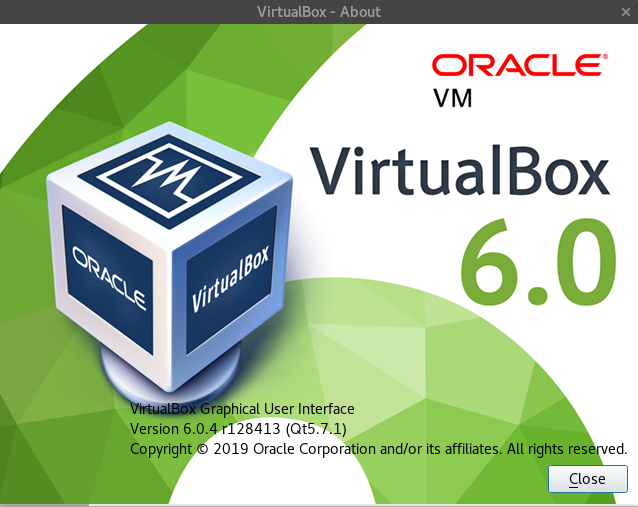
\includegraphics[scale=0.5]{Img/vbVersion.png}
\caption[loftitle]{Janela "Sobre" do Virtual Box - Oracle.}
\end{figure}

\textbf{Questão 3)}
\begin{figure}[!h]
\centering
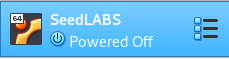
\includegraphics[scale=0.5]{Img/SeedInstall.png}
\caption[loftitle]{Máquina virtual com o disco do SEED Labs.}
\end{figure}

\textbf{Questão 4)} Disponível em \cite{michael}

\textbf{a)} cd, ls mkdir/rmdir

\textbf{b)} cp

\textbf{c)} cat

\textbf{d)} man, whais

\textbf{e)} top, kill -9 PID

\textbf{f)} top

\textbf{g)} chmod

\textbf{h)} tar

\textbf{i)} df

\textbf{j)} ssh e scp

\textbf{k)} apt-get ou dpkg


\textbf{Questão 5)} Usando o tutorial fornecido, segue o ip e ping na Figura 3


%Alterar o endereço IP seguindo o tutorial: http://www.cis.syr.edu/~wedu/seed/Labs_16.04/Documents/SEEDVM_VirtualBoxManual.pdf

\begin{figure}[!h]
\centering
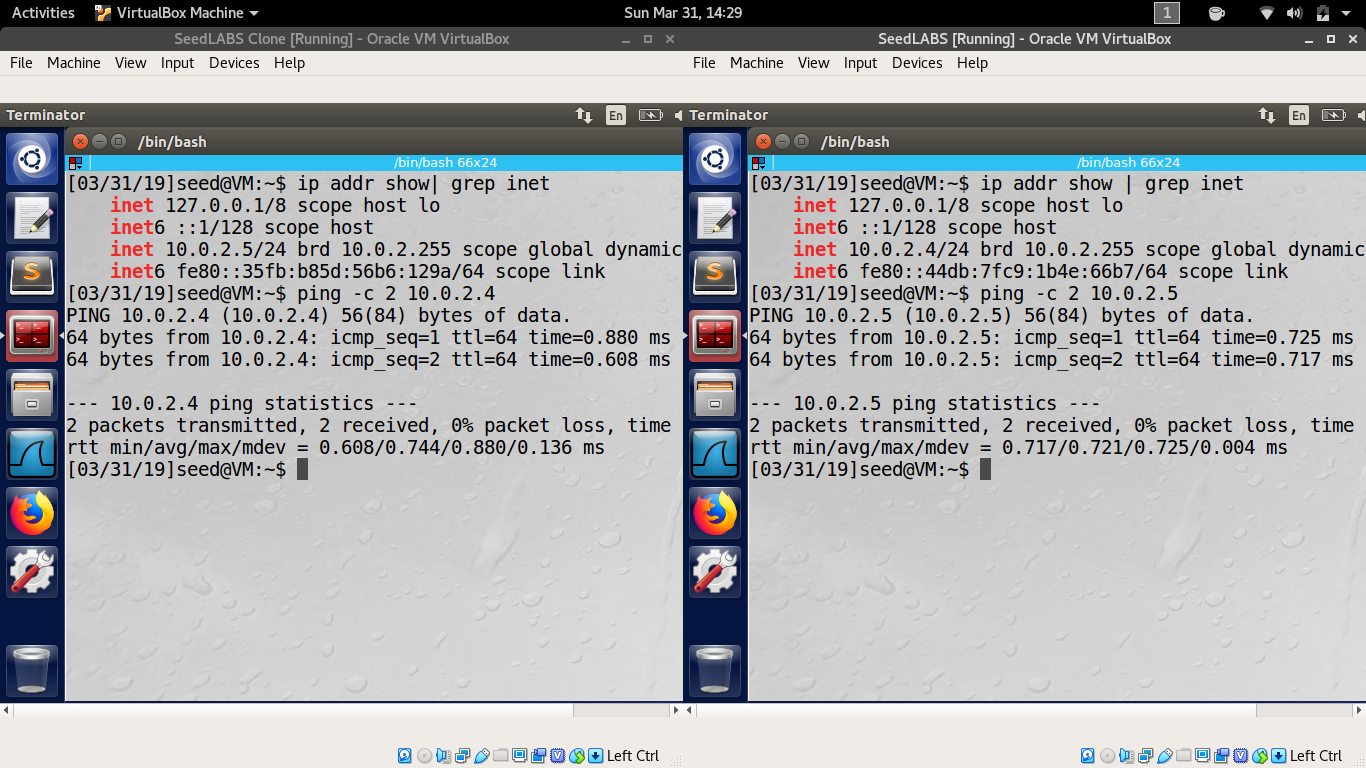
\includegraphics[scale=0.35]{Img/pingVb.png}
\label{IpPing}
\caption[loftitle]{Verificando o IP e usando PING para testar a conexão}
\end{figure}
\newpage
\textbf{Questão 6)}

Script1:
\lstinputlisting[language=bash]{script1.sh}

Script2: 
\lstinputlisting[language=bash]{script2.sh}

%Com base nos comandos recém aprendidos, crie dois bash/shell-scripts. O primeiro deve fornecer permissão de escrita/execução/leitura de um determinado diretório, compactá-lo e copiar o arquivo compactado para um diretório de sua escolha. O segundo bash script deve simular uma função de backup de arquivos. Ou seja, compactar diferentes arquivos, alterar o nome do arquivo de backup de acordo com o dia e a hora e enviar tal arquivo para outro computador.
%Incluir os scripts com o listings

\bibliographystyle{plain}
\bibliography{main}

\end{document}